\Chapter{Saját kód elhelyezése}

\Section{A MySQL adatbázis fordítása és telepítése}

A MySQL forráskódból való fordítását egy frissen telepített és naprakészre frissített Manjaro 20.2.1 es linux disztribúción végeztem el. Telepítés során non-free grafikus drivert választottam.
A forrásállomány bárki számára elérhető, és a következő paranccsal klónozható:
\begin{python}
 git clone https://github.com/mysql/mysql-server.git
\end{python}
A fordítás sikerességéhez rendszerenként eltérő csomagok telepítésére lehet szükség. Jelen esetben a következők telepítéseket igényelte a folyamat.
% QUEST: Miért snap-es csomaggal lett telepítve?
% ANSWER: A cmake telepítése a gyártó hivatalos weboldalán található Manjato rendszerhez készült segédlet alapján lett elvégezve.
\begin{python}
 $ sudo snap install cmake --classic
 $ sudo pacman -S rpcsvc-proto
 $ sudo pacman -S pkgconfig
 $ sudo pacman -S make
 $ sudo pacman -S gcc
 $ sudo pacman -S bison
\end{python}%$
%A \textit{Boost} függvénykönyvtár később kapcsoló használatával letölthető.
A következő lépés a CMake futtatása. Ehhez célszerű létrehozni egy mappát ahová az új állományok létrejöhetnek. Ezt nem kötelező megtenni, a forrás könyvtárban is ki lehet adni a parancsot, ehhez a \texttt{CMake} megfogja adni a szükséges kapcsolót illetve figyelmeztet arra, hogy nem ajánlatos.
\begin{python}
 mkdir build
\end{python}
Amint ez kész a forrás mappájában futtathatjuk a következő parancsot:
\begin{python}
 cmake ./ ../build -DDOWNLOAD_BOOST=1 -DWITH_BOOST=../boost/
\end{python}
A megadott kapcsolóval a boost könyvtár letöltődik a megadott helyre és a \texttt{CMake} megjegyez ezt. Ha a generátor hibába ütközik a szükséges csomagokat telepíteni kell és a \textit{CMakeCache.txt} fájlt törtölni. Ezek után a \texttt{CMake} újra futtatható, de már a \textit{Boost} -hoz tartozó kapcsolók nélkül.

A sikeres futás jelzi, hogy minden készen áll a fordításra, nincs hiányzó csomag.
A \texttt{make} parancs futtatása következik. Ez egy hosszú folyamat, jelen konfiguráción 120 percet vett igénybe. 

A sikeres fordítást követően létre kell hoznunk egy data mappát a szerver számára.
\begin{python}
 mkdir data
\end{python}
Első futtatást rendszergazdaként a megadott kapcsolóval kell végrehajtani, csak ekkor tudja a szerver létrehozni a fájljait!
\begin{python}
 sudo ./bin/mysqld --initialize
\end{python}
Ekkor kapunk egy jelszót az a szerverre való csatlakozáshoz. Következő futtatás előtt szükség lehet a data mappa jogosultságainak állítására, különben a szerver a normál indítás során nem tudja inicializálni az InnoDB-t olvasási hiba miatt.
\begin{python}
 sudo chmod -R 777 ./data
\end{python}
Ezután futtathatjuk a szervert
\texttt{./bin/mysqld}
Vagy telepíthetjük is azt a \texttt{make install} paranccsal, de ez jelen esetben szükségtelen.



Csatlakozás a szerverre:
\begin{python}
 ./bin/mysql -u root -p
\end{python}
A generált jelszó bemásolásával belépünk. Majd megváltoztatjuk a jelszót.
\begin{python}
ALTER USER 'root'@'localhost' IDENTIFIED BY 'uj jelszo';
\end{python}
Vagy használhatjuk a MySQL Workbench-et ami első belépéskor megkér minket a módosításra.
% TODO: SQL-es környezetet lesz majd célszerű használni helyette!


\Section{A MySQL Connector}

A \texttt{Connector}, \texttt{MySQL} alapszabványú drivereket biztosít különböző nyelveken, amelyek lehetővé teszik a fejlesztők számára, hogy adatbázis alkalmazásokat írjanak a támogatott nyelveken. Ezen kívül egy natív \texttt{C} könyvtár teszi lehetővé azt, hogy a \texttt{MySQL} -t közvetlenül beágyazhassák alkalmazásaikba. \newline
A következő \texttt{MySQL} által fejlesztett driverek érhetőek el: \newline
\texttt{ADO.NET}, \texttt{ODBC}, \texttt{JDBC}, \texttt{Node.js}, \texttt{Python}, \texttt{C++}, \texttt{C} és \texttt{C API} a klienshez. \newline
Az alábbiakat pedig a \texttt{MySQL} közössége fejleszti:\newline
\texttt{PHP}, \texttt{Perl}, \texttt{Ruby}, \texttt{C+ Wrapper}.

*https://www.mysql.com/products/connector/

\SubSection{A Connector/C++ használata}

Az állományok letölthetőek a készítő hivatalos weboldaláról:\newline
https://dev.mysql.com/downloads/connector/cpp/
\begin{itemize}
	\item Linux - Generic
	\item All
	\item Linux - Generic (glibc 2.12) (x86, 64-bit), Compressed TAR Archive
\end{itemize}
Letöltés után kicsomagoljuk. A tartalma egy \texttt{include} és egy \texttt{lib64} mappa. Az \texttt{include} mappa tartalmát a \texttt{usr/include} könyvtárba másoljuk, a \texttt{lib64} -ét pedig az \texttt{usr/lib64} mappába.

Ezután szükség lesz egy külön felhasználóra amellyel a program csatlakozni fog a szerverünkre. Ezt létrehozhatjuk a \texttt{Workbench} alkalmazásban is.
\begin{python}
	CREATE USER 'newuser'@'localhost' IDENTIFIED BY 'password';
\end{python}

\SubSection{Első program}

Hozzunk létre egy \texttt{connectortest.cpp} nevű fájlt.
Szükséges osztályok létrehozása:
\begin{cpp}
	sql::Driver *driver;
	sql::Connection *con;
	sql::Statement *stmt;
	sql::ResultSet *res;
	sql::PreparedStatement *pstmt;
\end{cpp}
Csatlakozás a szerverhez és adatbázis kiválasztása:
\begin{cpp}
	driver = get_driver_instance();
	con = driver->connect("tcp://192.168.0.43:3306", "program", "a");
	con->setSchema("thesis");
\end{cpp}
A következő két sor maga a lekérdezés. Az első utasítás elkészíti a szövegből a szerver számára is értelmezhető utasítást, a második sor pedig elküldi azt a szervernek és megvárja a választ:
\begin{cpp}
	pstmt = con->prepareStatement("SELECT * FROM T3");
	res = pstmt->executeQuery();
\end{cpp}

Az eredményt a \texttt{res} objektumon végig lépkedve tudjuk kiolvasni, a lekért oszlop nevének megadásával és a típusnak megfelelő \texttt{get} függvénynél.
\begin{cpp}
	while (res->next())
	cout << res->getInt("c1p3") << "\t" << res->getInt("c2") << "\t"
	<< res->getInt("c3") << "\t" << res->getInt("c4") << "\t"
	<< res->getInt("fk_p1_p3") << "\t" << res->getInt("fk_p2_p3") 
	<< endl;
\end{cpp}
Lekérdezés után fontos törölni az eredményhalmazt és az elkészített utasítást, ugyanis ezek memóriát foglalnak, és több lekérdezés esetén megtelhet akár a teljes memória is.
\begin{cpp}
	delete res;
	delete pstmt;
\end{cpp}
Futtatáshoz és fordításhoz a következő parancsokat használhatjuk: 
\begin{python}
	g++ -D_GLIBCXX_USE_CXX11_ABI=0 connectortest.cpp 
	-o connectortest.out -lmysqlcppconn
	
	./connectortest.out
\end{python}

\Section{Connector proxy létrehozása}

Azt feltételezhetjük, hogy a rendelkezésre álló MySQL elérési felületet érdemes megtartani valamilyen formában a lekérdezések optimalizálása során. Ez többek között az alábbiakkal indokolható.
\begin{itemize}
	\item A felület jól átgondolt, a területen járatos szakemberek készítették és a használat szempontjából kiállta az idő próbáját.
	\item Elterjedt. Amennyiben az a cél, hogy az elkészített szoftver előnyeit minél többen használni tudják, és akarják is, arra kell törekedni, hogy az új felhasználóknak minél kevesebb plusz munkát jelentsen az elsajátítása.
	\item Lehetőséget ad, hogy egy saját implementációval transzparens módon megoldható legyen az optimalizálás. Ez olyan szempontból kifejezetten praktikus, hogy így opcionálissá tehető az optimalizálási módszer használata. A szokványos és a dolgozatban bemutatásra kerülő OpenCL-el optimalizált elérés között a váltás kényelmesen megtehető.
\end{itemize}

A \textit{proxy} nevű tervezési minta kiválóan alkalmas lehet az említett feladat megoldására. \Aref{fig:proxy_arch}. ábrán bal oldal láthatjuk a hagyományos módszert, ahogy az adatokhoz hozzá lehet férni egy alkalmazásból. A jobb oldalt a proxy segítségével optimalizált változat látható.

\begin{figure}[h!]
\centering
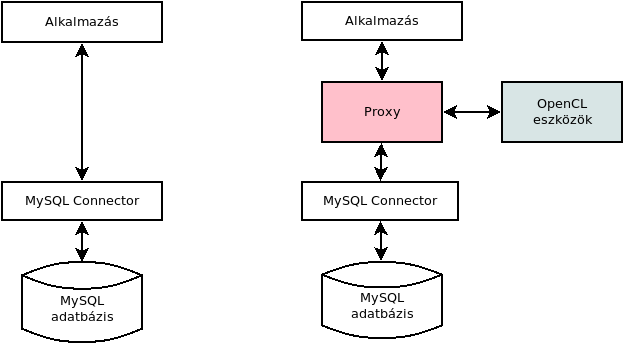
\includegraphics[width=\textwidth]{images/proxy_arch.png}
\caption{A hagyományos és az optimalizáláshoz használt proxy-val kiegészített felépítés}
\label{fig:proxy_arch}
\end{figure}

A feldolgozási folyamatot \aref{fig:process}. ábrán látható formában képzelhetjük el.

\begin{figure}[h!]
\centering
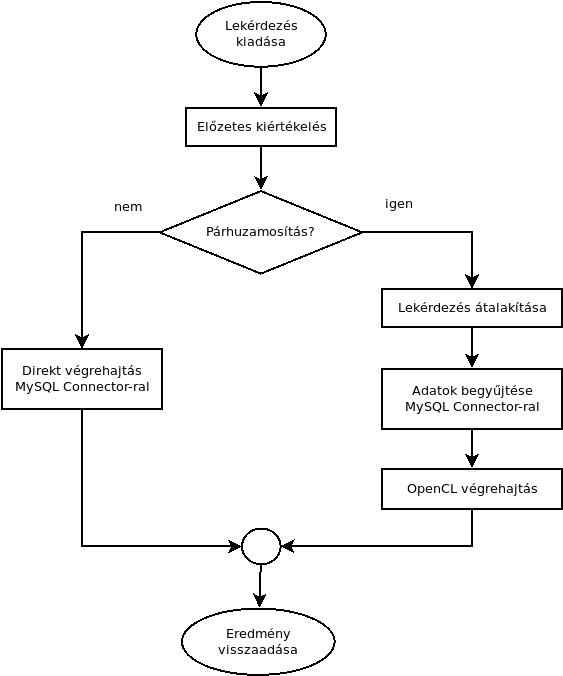
\includegraphics[width=\textwidth]{images/process.png}
\caption{A feldolgozási lépések a proxy beiktatásával}
\label{fig:process}
\end{figure}

Ennek az egyik igen fontos eleme az előzetes kiértékelő, amely a kapott lekérdezésről meg tudja állapítani, hogy azt érdemes-e párhuzamosítani.
\begin{itemize}
	\item Mivel ennek egy gyors döntést kell hoznia, a lekérdezést nem fogja végrehajtani, ezért csak egy becslést ad arra, hogy melyik végrehajtási mód lehet megfelelő.
	\item A kimenete egyszerűen csak egy logikai érték.
	\item Figyelembe kell vennie a lekérdezés összetettségét, az aktuálisan rendelkezésre álló számítási kapacitásokat, és adatbázisban lévő adatok mennyiségét.
	\item Adhatunk lehetőséget a felhasználónak, hogy direkt módon döntsön a feldolgozás menetéről. Ha a felhasználó ismeri a rendszer előnyeit, hátrányait olykor könnyedén dönthet arról, hogy használja -e az OpenCL-es kiértékelést. Például ha sok visszatérő sorrá számít akkor használja, ha nem biztos, akkor automatikus módban hagyja.
\end{itemize}

A következő fontos elem a lekérdezés átalakítása, amely a lekérdezést szétválasztja adatgyűjtési és kiértékelési részekre.
\begin{itemize}
	\item A párhuzamos végrehajtásnál úgy általában azt feltételezzük, hogy szelekciós műveletről van szó.
	\item Az adatgyűjtést követően már a számítási rész végrehajtásához nem szükséges az adatbázishoz fordulni.
\end{itemize}

Érdekes lehet egy olyan változatot is felvetni, amelyben a lekérdezés egyidejűleg elindul a direkt végrehajtás és a párhuzamos végrehajtás irányába is, majd azt az eredményt szolgáltatja, amelyik hamarabb visszatér. Ez elvi szinten ugyan megoldható, viszont feltételezhetően a konkurens végrehajtás miatt mindkét számítási idő sérülni fog az erőforráslimitek miatt. A későbbiekben tehát az előzetes kiértékelés eredményére hagyatkozhatunk.

\SubSection{Az API illesztése}

A dolgozat keretein belül nem cél a teljes Connector interfész megvalósítása, csak annak egy részhalmaza. Mivel proxy-ról van szó, ezért az összes olyan művelet átkötése mennyiségi problémát jelent csak, amely nem változtatja meg a végrehajtás módját.

A driver beállítások és az adatbázishoz kapcsolódás változatlan kell legyen, mivel azok szükségesek ahhoz, hogy hozzáférjünk az adatbázishoz.

A különbség a \texttt{prepareStatement} kapcsán jelenik meg. Ehhez kell tehát egy saját implementációt adni, amelyik kompatibilitási okokból származhat közvetlenül az \texttt{sql::PreparedStatement} osztályból. Hogy ha azt szeretnénk, hogy a kódban csak az \texttt{include}-okat kelljen megváltoztatni, akkor érdemes a \texttt{Driver} és \texttt{Connection} osztályokat szintén származtatni. Mivel az interfész megtartható, ezért statikus linkeléssel is lehetőség adódhat a funkció cseréjére, vagyis hogy a fejlesztő (mint célfelhasználó) a saját alkalmazásához nem a \texttt{Connector}-t fogja használni, hanem a proxy-t (amely aztán használja a \texttt{Connector}-t).


